\documentclass[a4paper, 12pt]{article}
\usepackage[a4paper,top=1.5cm, bottom=1.5cm, left=1cm, right=1cm]{geometry}
\usepackage{cmap}					% поиск в PDF
\usepackage{mathtext} 				% русские буквы в фомулах
\usepackage[T2A]{fontenc}			% кодировка
\usepackage[utf8]{inputenc}			% кодировка исходного текста
\usepackage[english,russian]{babel}	% локализация и переносы

\usepackage{amsmath}
\usepackage{indentfirst}
\usepackage{longtable}
\usepackage{graphicx}
\usepackage{array}

\usepackage{wrapfig}
\usepackage{siunitx} % Required for alignment
\usepackage{subfigure}
\usepackage{multirow}
\usepackage{rotating}
\usepackage{caption}

\graphicspath{{.}}


\title{\begin{center}Лабораторная работа №2.1.4\end{center}
Определение теплоемкости твердых тел}
\author{Рожков А. В. \\ Преподаватель Яворский В. А.}
\date{\today}

\begin{document}
    \pagenumbering{gobble}
    \maketitle
    \newpage
    \pagenumbering{arabic}

    \textbf{Цель работы:} измерение количества подведенного тепла и вызванного им нагрева твердого тела; определение теплоемкости по экстраполяции отношения $\Delta Q / \Delta T$ к нулевым потерям тепла.

	\textbf{В работе используются:} калориметр с нагревателем и термометром сопротивления; амперметр; вольтметр; мост постоянного тока; источник питания 36 В.

    \section{Теоретическая справка}

    В данной работе теплоемкость определяется по формуле
    \begin{equation}
        C = \frac{\Delta Q}{\Delta T},
        \label{eq:dQdT}
    \end{equation}

    где $\Delta Q$ -- количество тепла, подведенного к телу, и $\Delta T$ -- изменение температуры тела, произошедшее в результате подвода тепла.

    Температура исследуемого тела надежно измеряется термометром сопротивления, а определение количества тепла, поглощенного телом, обычно вызывает затруднение. В реальных условиях не вся энергия $P \Delta t$, выделенная нагревателем, идет на нагревание исследуемого тела и калориметра, часть ее уходит из калориметра благодаря теплопроводности его стенок. Оставшееся в калориметре количество тепла $\Delta Q$ равно
    \begin{equation}
        \Delta Q = P\Delta t - \lambda(T - T_{\text{к}}) \Delta t,
        \label{eq:dQ}
    \end{equation}
    где $P$ -- мощность нагревателя, $\lambda$ -- коэффициент теплоотдачи стенок, $T$ -- температура тела, $T_{\text{к}}$ -- комнатная температура, $ \Delta t$ -- время, в течение которого идет нагревание.

    Из уравнений (1) и (2) получаем
    \begin{equation}
        C = \frac{P - \lambda(T - T_{\text{к}})}{\Delta T / \Delta t}
        \label{osnovnaya}
    \end{equation}
    Формула (3) является основной расчетной формулой. Она определяет теплоемкость тела вместе с калориметром. Теплоемкость калориметра измеряется отдельно и вычитается из результата.

    С увеличением температуры исследуемого тела растет утечка энергии, связанная с теплопроводностью стенок калориметра. Из формулы (2) видноб что при постоянной мощности нагревателя по мере роста температуры количество теплаб передаваемое телу, уменьшается, и, следовательно, понижается скорость изменения его температуры.

    Погрешности, связанные с утечкой тепла, оказываются небольшими, если не давать телу заметных перегревов и проводить все измерения при температурах, мало отличающихся от комнатной. Однако при небольших перегревах возникает большая ошибка при измерении $\Delta T = T - T_\text{к}$, и точность определения теплоемкости не возрастает. Чтобы избежать этой трудности, в работе используется следующая методика измерений. Зависимость скорости нагревания тела $\Delta T / \Delta t$ от температуры измеряется в широком интервале изменения температур. По полученным данным строится график
    \begin{equation*}
        \frac{\Delta T}{\Delta t} = f(T).
    \end{equation*}
    Этот график экстраполируется к температуре $T = T_{\text{к}}$, и таким образом определяется скорость нагревания при комнатной температуре $(\Delta T / \Delta t)_{T_{\text{к}}}$. Подставляя полученное выражение в формулу (3) и замечая, что при $T = T_{\text{к}}$ член $\lambda(T - T_{\text{к}})$ обращается в ноль, получаем
    \begin{equation}
        C = \frac{P}{(\Delta T / \Delta t)_{T_{\text{к}}}}
        \label{4}
    \end{equation}


    \begin{figure}[h]
        \centering
        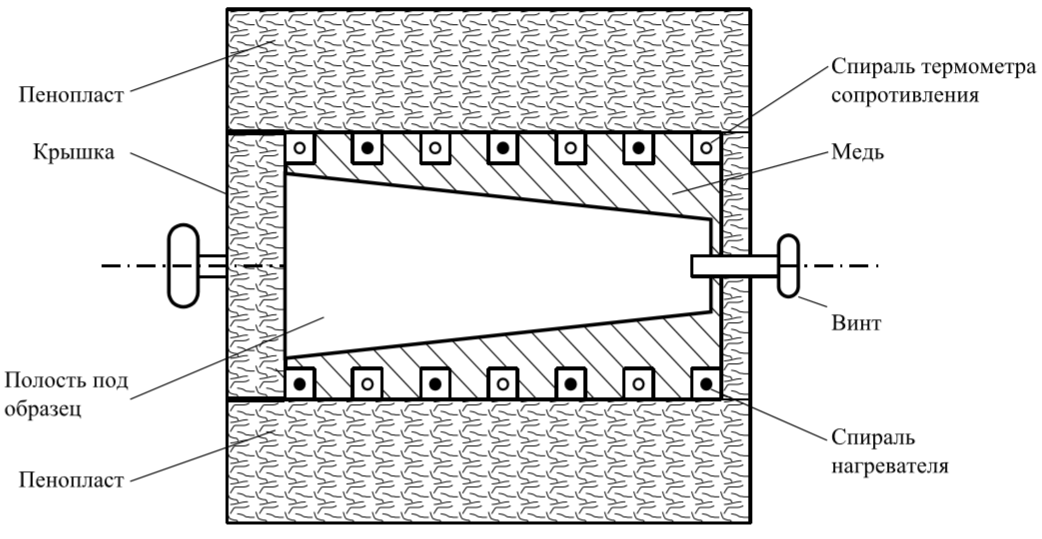
\includegraphics[width=0.8\textwidth]{img/calorimeter.png}
        \caption{Схема устройства калориметра}
        \label{fig:calorimeter}
    \end{figure}

    Температура измеряется термометром сопротивления, который представляет собой медную проволоку, намотанную на теплопроводящий каркас внутренней стенки калориметра (рис. 1). Сопротивление проводника изменяется с температурой по закону

    \begin{equation}
        R_{T} = R_{0}(1 + \alpha \Delta T),
        \label{RT}
    \end{equation}

    где $R_{T}$ -- сопротивление термеметра про $T  ^{\circ}C$, $R_{0}$ -- его сопротивление при $0  ^{\circ}C$, $\alpha$ -- температурный коэффициент сопротивления.

    Дифференцируя (5) по времени, найдем

    \begin{equation}
        \frac{dR}{dt} = R_{0}\alpha \frac{dT}{dt},
        \label{dRT}
    \end{equation}

    Выразим сопротивление $R_{0}$ через исмеренное значение $R_{\text{к}}$ -- сопротивление термометра при комнатной температуре. Согласно (5), имеем

    \begin{equation}
        R_{0} = \frac{R_{\text{к}}}{1 + \alpha \Delta T_{\text{к}}},
        \label{R0}
    \end{equation}

    Подставляя (6) и (7) в (4), найдем

    \begin{equation}
        C = \frac{PR_{\text{к}} \alpha}{(\frac{dR}{dt})_{T_{\text{к}}}(1 + \alpha \Delta T_{\text{к}})},
        \label{capacity}
    \end{equation}

    Входящий в формулу температурный коэффициент сопротивления меди $\alpha = 4,28 \cdot 10^{-3}~{^oC}^{-1}$, все остальные величины определяются экспериментально.

    \subsection*{Экспериментальная установка}

    Установка состоит из калориметра с пенопластовой изоляцией, помещенного в ящик из многослойной клееной фанеры. Внутренние стенки калориметра выполненым из материала с высокой теплопроводностью. Надежность теплового контакта между телом и стенками обеспечивается их формой: они имеют вид усеченных конусов и плотно прилегают друг к другу. В стенку калориметра вмонтированы электронагреватель и термометр сопротивления. Схема включения нагревателя изображения на рис.2. Система реостатов позволяет установить нужную силу тока в цепи нагревателя. По амперметру и вольтметру определяется мощность, выделяемая в нагревателе. Величина сопротивления термометра измеряется мостом постоянного тока.

    \begin{figure}[!h]
        \centering
        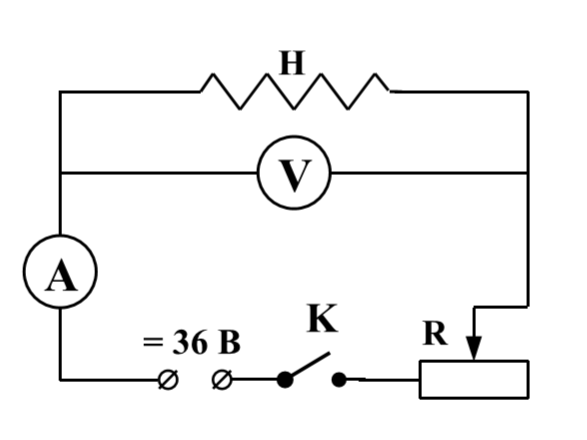
\includegraphics[width=0.4\textwidth]{"img/heater.png"}
        \caption{Схема включения нагревателя}
        \label{fig:boiler}
    \end{figure}



\end{document}
